\documentclass[10pt]{exam}
\usepackage[hon]{template-for-exam}
\usepackage{graphicx}

\title{Work-Kinetic Energy Problems}
\author{Rohrbach}
\date{\today}

\begin{document}
\maketitle

\begin{questions}
  \question How much work must be done to stop a 925-kg car traveling at 26~m/s?
  \vs
  \question A 0.085-kg arrow is fired from a bow whose string exerts an average force of 105~N on the arrow over a distance of 75~cm. What is the speed of the arrow as it leaves the bow?
  \vs
  \pagebreak
  \question A 380-kg piano slides 2.9 m down a 25° incline and is kept from accelerating by a man who is pushing back on it parallel to the incline. Determine: (a) the force exerted by the man, (b) the work done on the piano by the man, (c) the work done on the piano by the force of gravity, and (d) the net work done on the piano. Ignore friction.

  \vspace{2em}

  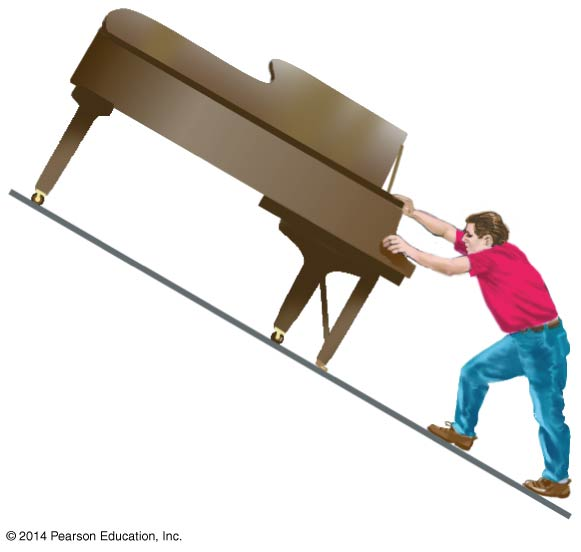
\includegraphics[width=4cm]{./figures/06_36_Figure.jpg}




  \vs

  {\small These problems are taken from Giancolli \emph{Physics: Principles with Applications}, Chapter 6.}

\end{questions}

\end{document}